
\documentclass[10pt]{article}

\usepackage[a4paper,margin=0.65in]{geometry}
\usepackage{amsmath,amssymb}
\usepackage{graphicx}
\usepackage{booktabs}
\usepackage{array}
\usepackage{float}
\usepackage{hyperref}
\usepackage{enumitem}
\usepackage{xcolor}
\usepackage{tikz}
\usetikzlibrary{positioning,arrows.meta,shapes.geometric,fit,calc}

\setlist{nosep,leftmargin=*}
\renewcommand{\arraystretch}{1.2}
\setlength{\parindent}{0pt}
\setlength{\parskip}{2pt}

\tikzset{
layer/.style={
draw,
rounded corners,
minimum width=1.7cm,
minimum height=0.65cm,
align=center,
fill=blue!10,
font=\scriptsize
},
smalllayer/.style={
draw,
rounded corners,
minimum width=1.35cm,
minimum height=0.58cm,
align=center,
fill=green!10,
font=\scriptsize
},
arrow/.style={
-{Latex[length=2mm]},
thin
}
}

\begin{document}

%%%%%%%%%%%%%%%%%%%%%%%%%%%%%%%%%%%%%%%%%%%%%%%%%%%%%%%%%%%%
% TITLE
%%%%%%%%%%%%%%%%%%%%%%%%%%%%%%%%%%%%%%%%%%%%%%%%%%%%%%%%%%%%

\begin{center}

{\large\textbf{Shiv Nadar University Chennai}}

\vspace{2mm}

{\normalsize\textbf{CS3807 -- Deep Learning Laboratory}}

\vspace{2mm}

{\large\textbf{Experiment 7}}

\vspace{1mm}

{\normalsize\textbf{End-to-End Study of Autoencoders, Convolutional}}

{\normalsize\textbf{Autoencoders, Denoising Autoencoders and Variational Autoencoders}}

\end{center}

\vspace{3mm}

\begin{tabular}{|p{3.4cm}|p{9.0cm}|p{1.4cm}|}
\hline
Degree \& Branch &
B.Tech Artificial Intelligence \& Data Science &
Semester V\\
\hline
Subject Code \& Name &
CS3807 -- Deep Learning Laboratory &
AY: 2026--27\\
\hline
\end{tabular}

%%%%%%%%%%%%%%%%%%%%%%%%%%%%%%%%%%%%%%%%%%%%%%%%%%%%%%%%%%%%
\section*{1. Objective}

The objective of this experiment is to develop an end-to-end understanding of
autoencoders and their variants for image representation, reconstruction,
denoising and generative modeling.

The experiment begins with a fully connected autoencoder, progresses to a
Convolutional Autoencoder (CAE), introduces image corruption for denoising,
and finally develops a Variational Autoencoder (VAE). Students will visualize
the learned latent representation, compare reconstruction quality using
quantitative and qualitative measures, and explore the generative capability
of the VAE.

The same image dataset and a controlled experimental protocol should be used
throughout the experiment wherever possible.

%%%%%%%%%%%%%%%%%%%%%%%%%%%%%%%%%%%%%%%%%%%%%%%%%%%%%%%%%%%%
\section*{2. Learning Outcomes}

After completing this experiment, students will be able to:

\begin{itemize}
\item explain the encoder--latent--decoder structure of an autoencoder;
\item prepare image data for reconstruction-based learning;
\item implement a fully connected autoencoder;
\item implement a Convolutional Autoencoder for image reconstruction;
\item introduce controlled noise and build a denoising autoencoder;
\item evaluate reconstruction using MSE, MAE and SSIM;
\item visualize and interpret latent representations;
\item explain the probabilistic latent representation of a VAE;
\item implement the reparameterization trick;
\item calculate and interpret reconstruction and KL-divergence losses;
\item generate new images by sampling from a learned latent space; and
\item compare deterministic and variational latent representations.
\end{itemize}

%%%%%%%%%%%%%%%%%%%%%%%%%%%%%%%%%%%%%%%%%%%%%%%%%%%%%%%%%%%%
\section*{3. Dataset and Experimental Setup}

\textbf{Dataset: MNIST Handwritten Digit Dataset}

MNIST contains grayscale images of handwritten digits from 0 to 9. Each image
has spatial dimensions

\[
28\times28\times1.
\]

The dataset is particularly suitable for this experiment because the images
are small, the classes have visually meaningful structure, and the same image
format can be directly supplied to fully connected, convolutional and
variational autoencoders.

The dataset can be loaded directly using Keras/TensorFlow:

\url{https://www.tensorflow.org/api_docs/python/tf/keras/datasets/mnist}

\textbf{Recommended laboratory subset:}

Use 10,000 training images and 2,000 test images for the main laboratory
execution. The full MNIST dataset may be used if computational resources
permit.

The labels are not required as reconstruction targets. The original image is
the target:

\[
\boxed{x\rightarrow \text{Encoder}\rightarrow z
\rightarrow\text{Decoder}\rightarrow\hat{x}}
\]

where $x$ is the input image and $\hat{x}$ is its reconstruction.

%%%%%%%%%%%%%%%%%%%%%%%%%%%%%%%%%%%%%%%%%%%%%%%%%%%%%%%%%%%%
\section*{4. Expected Input and Output}

\subsection*{Expected Input}

Each input image has shape

\[
28\times28\times1.
\]

For a batch of 32 images:

\[
X\in\mathbb{R}^{32\times28\times28\times1}.
\]

Pixel values should be converted from

\[
[0,255]\rightarrow[0,1].
\]

For a fully connected autoencoder, the image may be flattened:

\[
28\times28=784.
\]

Therefore,

\[
x\in\mathbb{R}^{784}.
\]

For a convolutional autoencoder, retain the spatial structure:

\[
x\in\mathbb{R}^{28\times28\times1}.
\]

\subsection*{Expected Output}

The primary output is a reconstructed image:

\[
\hat{x}\in\mathbb{R}^{28\times28\times1}.
\]

Students must display:

\begin{verbatim}
Original image
Reconstructed image
Reconstruction error
\end{verbatim}

For the denoising model, display:

\begin{verbatim}
Original clean image
Noisy image
Denoised reconstruction
\end{verbatim}

For the VAE, display newly generated samples obtained by sampling from the
latent distribution.

\begin{figure}[H]
    
    \includegraphics[width=\textwidth]{1.png}
    \caption{Original, reconstructed images and reconstruction error.}
\end{figure}

\begin{figure}[H]
   
    \includegraphics[width=\textwidth]{2.png}
    \caption{Clean, noisy and denoised images.}
\end{figure}
\begin{figure}[H]
    \centering
    \includegraphics[width=\textwidth]{3.png}
    \caption{VAE-generated samples obtained by sampling from the latent distribution.}
\end{figure}
%%%%%%%%%%%%%%%%%%%%%%%%%%%%%%%%%%%%%%%%%%%%%%%%%%%%%%%%%%%%
\section*{5. Overall Experimental Pipeline}

The complete experiment follows:

\begin{center}
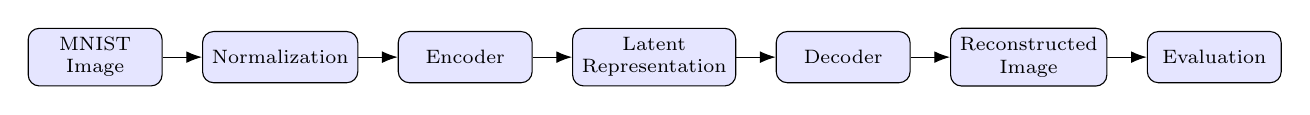
\begin{tikzpicture}[node distance=5mm]
\node[layer](a){MNIST\\Image};
\node[layer,right=of a](b){Normalization};
\node[layer,right=of b](c){Encoder};
\node[layer,right=of c](d){Latent\\Representation};
\node[layer,right=of d](e){Decoder};
\node[layer,right=of e](f){Reconstructed\\Image};
\node[layer,right=of f](g){Evaluation};

\foreach \x/\y in {a/b,b/c,c/d,d/e,e/f,f/g}
\draw[arrow](\x)--(\y);
\end{tikzpicture}
\end{center}

The experiment consists of four related studies:

\begin{enumerate}
\item Fully Connected Autoencoder
\item Convolutional Autoencoder
\item Denoising Convolutional Autoencoder
\item Variational Autoencoder
\end{enumerate}

%%%%%%%%%%%%%%%%%%%%%%%%%%%%%%%%%%%%%%%%%%%%%%%%%%%%%%%%%%%%
\section*{6. Exploring Autoencoders}

An autoencoder learns to reproduce its input at the output.

The encoder maps the input to a lower-dimensional representation:

\[
z=f_{\theta}(x),
\]

and the decoder reconstructs the input:

\[
\hat{x}=g_{\phi}(z).
\]

The training objective is to minimize reconstruction error:

\[
\mathcal{L}_{rec}
=
\frac{1}{N}\sum_{i=1}^{N}
\|x_i-\hat{x}_i\|^2.
\]

\begin{center}
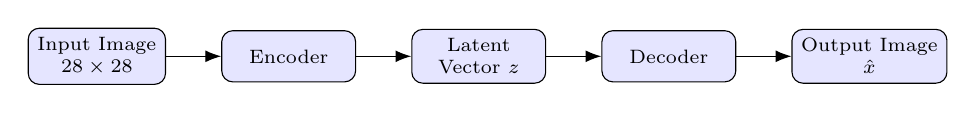
\begin{tikzpicture}[node distance=7mm]
\node[layer](a){Input Image\\$28\times28$};
\node[layer,right=of a](b){Encoder};
\node[layer,right=of b](c){Latent\\Vector $z$};
\node[layer,right=of c](d){Decoder};
\node[layer,right=of d](e){Output Image\\$\hat{x}$};

\foreach \x/\y in {a/b,b/c,c/d,d/e}
\draw[arrow](\x)--(\y);
\end{tikzpicture}
\end{center}

The latent vector is a compressed representation of the input.

%%%%%%%%%%%%%%%%%%%%%%%%%%%%%%%%%%%%%%%%%%%%%%%%%%%%%%%%%%%%
\section*{7. Fully Connected Autoencoder}

Flatten each image from

\[
28\times28=784
\]

to a vector of length 784.

Use the following architecture:

\begin{center}
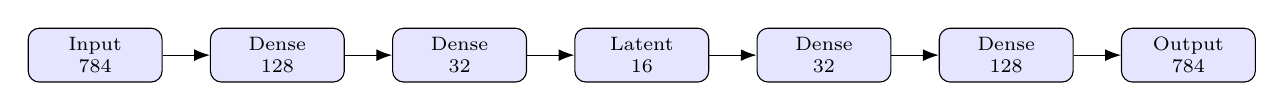
\begin{tikzpicture}[node distance=6mm]
\node[layer](a){Input\\784};
\node[layer,right=of a](b){Dense\\128};
\node[layer,right=of b](c){Dense\\32};
\node[layer,right=of c](d){Latent\\16};
\node[layer,right=of d](e){Dense\\32};
\node[layer,right=of e](f){Dense\\128};
\node[layer,right=of f](g){Output\\784};

\foreach \x/\y in {a/b,b/c,c/d,d/e,e/f,f/g}
\draw[arrow](\x)--(\y);
\end{tikzpicture}
\end{center}

Use ReLU activation in hidden layers and sigmoid activation in the output
layer.

\textbf{Suggested configuration:}

\begin{center}
\begin{tabular}{|l|l|}
\hline
Parameter & Value\\
\hline
Latent dimension & 16\\
Optimizer & Adam\\
Learning rate & $10^{-3}$\\
Batch size & 128\\
Epochs & 20\\
Loss & Binary Cross-Entropy\\
\hline
\end{tabular}
\end{center}

%%%%%%%%%%%%%%%%%%%%%%%%%%%%%%%%%%%%%%%%%%%%%%%%%%%%%%%%%%%%
\section*{8. Required Analysis of the Basic Autoencoder}

\textbf{Plot 1: Original versus Reconstructed Images}

Display at least 10 test images in a grid.

For every image, show:

\[
\text{Original}\quad|\quad\text{Reconstruction}.
\]

Students must comment on:

\begin{itemize}
\item preservation of digit shape;
\item loss of fine details;
\item blurred regions;
\item differences between easy and difficult samples.
\end{itemize}

\textbf{Plot 2: Training and Validation Reconstruction Loss}

\begin{itemize}
\item X-axis: Epoch
\item Y-axis: Reconstruction loss
\item Curves: Training loss and validation loss
\end{itemize}

\textbf{Required inference:} Determine whether the model converges and whether
there is evidence of overfitting.
\begin{figure}[H]
    \centering
    \includegraphics[width=\textwidth]{4.png}
    \caption{Plot 1: Original versus reconstructed images.}
\end{figure}

\textbf{Inference:} In this graph, one can observe the original MNIST images and their reconstruction. The basic structures of the digits have been retained by and large, indicating that the autoencoder is capable of capturing the basic structure of the digits. However, some minor details have been lost, and there is an observable blurring effect in the reconstruction of some digits. The simpler digits are reconstructed more accurately than the complex ones.
\begin{figure}[H]
    \centering
    \includegraphics[width=\textwidth]{5.png}
    \caption{Plot 2: Training and validation reconstruction loss.}
\end{figure}

\textbf{Inference:}In this case, the figure presents the evolution of the reconstruction losses for the training and validation processes for 20 epochs. In both cases, the loss falls fast at the beginning and later slowly decreases, which suggests that the network is learning and converging. The training and validation losses do not diverge from each other significantly during training. It means that there is no indication of overfitting.

\begin{figure}[H]
    \centering
    \includegraphics[width=0.8\textwidth]{6.png}
    \caption{Example of absolute reconstruction error between the original and reconstructed image.}
\end{figure}

\textbf{Inference:}This reconstruction error image represents the pixels on which there are reconstruction differences between the image and the actual digit. There are maximum differences where the reconstructed digit is blurred or the shape is different from the original one. These differences exist along the strokes and boundaries of the digit. Those pixels at which there are fewer differences can be considered those that have less reconstruction error. This proves that there is a relationship between reconstruction error and visual differences.
%%%%%%%%%%%%%%%%%%%%%%%%%%%%%%%%%%%%%%%%%%%%%%%%%%%%%%%%%%%%
\section*{9. Reconstruction Metrics}

Students must calculate the following metrics on the test set.

\subsection*{Mean Squared Error}

\[
MSE=
\frac{1}{N}
\sum_{i=1}^{N}
(x_i-\hat{x}_i)^2.
\]

\subsection*{Mean Absolute Error}

\[
MAE=
\frac{1}{N}
\sum_{i=1}^{N}
|x_i-\hat{x}_i|.
\]

\subsection*{Structural Similarity}

Calculate SSIM between the original and reconstructed images.

The implementation may use:

\url{https://scikit-image.org/docs/stable/api/skimage.metrics.html}

Report:
\begin{center}
\begin{tabular}{|l|c|}
\hline
\textbf{Metric} & \textbf{Value}\\
\hline
Test MSE & 0.022764\\
Test MAE & 0.060162\\
Mean SSIM & 0.724705\\
\hline
\end{tabular}
\end{center}

\textbf{Inference:} The Fully Connected Autoencoder achieved a test MSE of 0.022764 and a test MAE of 0.060162, indicating relatively small average reconstruction errors. The Mean SSIM of 0.724705 shows that the reconstructed images preserve a substantial amount of the structural information present in the original MNIST images. The results are consistent with the visual reconstructions, where the main digit shapes are preserved but some fine details and boundaries are slightly blurred. Overall, the metrics indicate that the autoencoder is able to reconstruct the test images reasonably well while some pixel-level and structural differences remain.
%%%%%%%%%%%%%%%%%%%%%%%%%%%%%%%%%%%%%%%%%%%%%%%%%%%%%%%%%%%%
\section*{10. Convolutional Autoencoder}

A Convolutional Autoencoder preserves spatial structure and uses convolutional
operations in the encoder and upsampling/transposed convolution operations
in the decoder.

The conceptual architecture is:

\begin{center}
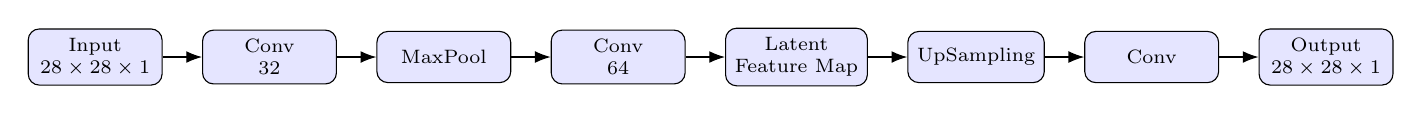
\begin{tikzpicture}[node distance=5mm]
\node[layer](a){Input\\$28\times28\times1$};
\node[layer,right=of a](b){Conv\\32};
\node[layer,right=of b](c){MaxPool};
\node[layer,right=of c](d){Conv\\64};
\node[layer,right=of d](e){Latent\\Feature Map};
\node[layer,right=of e](f){UpSampling};
\node[layer,right=of f](g){Conv};
\node[layer,right=of g](h){Output\\$28\times28\times1$};

\foreach \x/\y in {a/b,b/c,c/d,d/e,e/f,f/g,g/h}
\draw[arrow](\x)--(\y);
\end{tikzpicture}
\end{center}

A possible implementation is:

\begin{verbatim}
Input(28,28,1)
Conv2D(32, 3, activation='relu', padding='same')
MaxPooling2D(2, padding='same')
Conv2D(64, 3, activation='relu', padding='same')
MaxPooling2D(2, padding='same')
Conv2D(64, 3, activation='relu', padding='same')
UpSampling2D(2)
Conv2D(32, 3, activation='relu', padding='same')
UpSampling2D(2)
Conv2D(1, 3, activation='sigmoid', padding='same')
\end{verbatim}

The exact implementation may use Conv2DTranspose instead of UpSampling2D.

%%%%%%%%%%%%%%%%%%%%%%%%%%%%%%%%%%%%%%%%%%%%%%%%%%%%%%%%%%%%
\section*{11. Comparing Fully Connected and Convolutional Autoencoders}

Train both models using the same training and test images.


\begin{center}
\begin{tabular}{|l|c|c|c|c|}
\hline
\textbf{Model} & \textbf{MSE} & \textbf{MAE} & \textbf{SSIM} & \textbf{Parameters}\\
\hline
Fully Connected AE & 0.022764 & 0.060162 & 0.724705 & 211040\\
Convolutional AE & 0.002618 & 0.015085 & 0.973805 & 74497\\
\hline
\end{tabular}
\end{center}


\textbf{Plot 3: Reconstruction Comparison}

Display:

\[
\text{Original}
\rightarrow
\text{FC-AE Reconstruction}
\rightarrow
\text{CAE Reconstruction}.
\]
\begin{figure}[H]
    \centering
    \includegraphics[width=0.9\textwidth]{7.png}
    \caption{Plot 3: Original image compared with FC-AE and CAE reconstructions.}
\end{figure}
\textbf{Inference:}The graph displays the original image, along with the images that have been reconstructed using the Fully Connected Autoencoder and the Convolutional Autoencoder. CAE reconstructs an image more accurately with its digits shape intact, compared to the FC-AE, which has a relatively blurred reconstruction. This is due to the fact that convolution layers retain the spatial locality and learn patterns locally such as edges and strokes, while the FC-AE does not retain the spatial locality of pixels since it works on the flattened pixels without any consideration of their spatial locality. The quantified values confirm this statement in that the MSE of the CAE is 0.002618, MAE is 0.015085, and the SSIM is 0.973805 compared to the FC-AE.

%%%%%%%%%%%%%%%%%%%%%%%%%%%%%%%%%%%%%%%%%%%%%%%%%%%%%%%%%%%%
\section*{12. Denoising Autoencoder}

A denoising autoencoder receives a corrupted image but is trained to
reconstruct the original clean image.

The training mapping is:

\[
\boxed{\tilde{x}\rightarrow\text{Encoder}\rightarrow z
\rightarrow\text{Decoder}\rightarrow\hat{x}}
\]

where $\tilde{x}$ is a noisy version of the clean image $x$.

\begin{center}
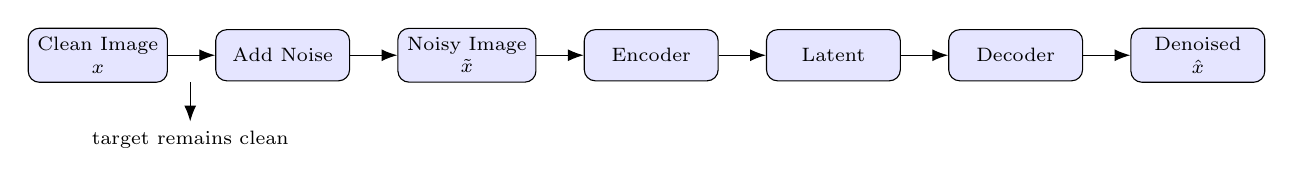
\begin{tikzpicture}[node distance=6mm]
\node[layer](a){Clean Image\\$x$};
\node[layer,right=of a](b){Add Noise};
\node[layer,right=of b](c){Noisy Image\\$\tilde{x}$};
\node[layer,right=of c](d){Encoder};
\node[layer,right=of d](e){Latent};
\node[layer,right=of e](f){Decoder};
\node[layer,right=of f](g){Denoised\\$\hat{x}$};

\foreach \x/\y in {a/b,b/c,c/d,d/e,e/f,f/g}
\draw[arrow](\x)--(\y);

\draw[arrow]($(a.south)!0.5!(b.south)$) -- ++(0,-5mm)
node[below,font=\scriptsize]{target remains clean};
\end{tikzpicture}
\end{center}

%%%%%%%%%%%%%%%%%%%%%%%%%%%%%%%%%%%%%%%%%%%%%%%%%%%%%%%%%%%%
\section*{13. Adding Image Noise}

Use at least two corruption types.

\subsection*{Gaussian Noise}

\[
\tilde{x}=x+n,
\qquad
n\sim\mathcal{N}(0,\sigma^2).
\]

Suggested standard deviations:

\[
\sigma\in\{0.1,0.2,0.3\}.
\]

Clip the resulting image to the range $[0,1]$.

\subsection*{Salt-and-Pepper Noise}

Randomly replace a small proportion of pixels with values close to 0 or 1.

Suggested corruption levels:

\[
p\in\{0.05,0.10,0.20\}.
\]

%%%%%%%%%%%%%%%%%%%%%%%%%%%%%%%%%%%%%%%%%%%%%%%%%%%%%%%%%%%%
\section*{14. Required Denoising Plots}

\textbf{Plot 4: Clean vs. Noisy vs. Denoised}

For at least 10 images, display:

\[
\text{Clean}\quad|\quad
\text{Noisy}\quad|\quad
\text{Denoised}.
\]
\begin{figure}[H]
    \centering
    \includegraphics[width=0.7\textwidth]{8.png}
    \caption{Plot 4: Clean, noisy, and denoised images.}
\end{figure}

\textbf{Inference:} As shown by the plot below, it has been demonstrated through the use of clean MNIST images, their version with the addition of noise and the reconstruction of the same without noise. It is clear that the images with the added noise have pixel-level corruption, while those without it capture the essential form and strokes of the original images. Even though some finer details may be lost, the fundamental forms of the digits are retained.

\textbf{Plot 5: Noise Level vs. Reconstruction Quality}

For each noise level, calculate:

\[
MSE,\quad MAE,\quad SSIM.
\]

Report:
\begin{center}
\begin{tabular}{|c|c|c|c|}
\hline
\textbf{Noise Level} & \textbf{MSE} & \textbf{MAE} & \textbf{SSIM}\\
\hline
0.1 & 0.003628 & 0.017821 & 0.959859\\
0.2 & 0.004630 & 0.021293 & 0.944413\\
0.3 & 0.007102 & 0.029666 & 0.863580\\
\hline
\end{tabular}
\end{center}


\textbf{Inference:}In the story, there are original MNIST images, MNIST images that have been affected by addition of noise, and finally the images after de-noising the images. In the images with noise, we observe that there are many pixel distortions, but in the images after de-noising, we can notice that the original structure and lines of the images have been restored. Although we have lost some details and smoothness, the structure has remained intact. Therefore, we can conclude that the denoising autoencoder knows how to de-noise the images.

\begin{figure}[H]
    \centering
    \includegraphics[width=0.75\textwidth]{9.png}
    \caption{Plot 5A: Gaussian noise level versus reconstruction MSE.}
\end{figure}

\textbf{Inference:} The graph demonstrates the dependency between the level of Gaussian noise and the MSE of reconstruction. The MSE is rising from 0.003628 for $\sigma=0.1$, to 0.004630 for $\sigma=0.2$ and to 0.007102 for $\sigma=0.3$. That means that the higher level of Gaussian noise causes higher error in reconstruction. With increasing level of noise the image gets higher corruption and becomes harder to reconstruct because of that.

\begin{figure}[H]
    \centering
    \includegraphics[width=0.75\textwidth]{10.png}
    \caption{Plot 5B: Gaussian noise level versus reconstruction MAE.}
\end{figure}

\textbf{Inference:} From the above results, the plot depicts an increase in the reconstruction MAE as the level of noise in the Gaussian increases. In this case, the MAE changes from 0.017821 when the $\sigma$ is 0.1 to 0.021293 when $\sigma$ is 0.2 and then 0.029666 when $\sigma$ is 0.3. This happens due to the fact that increased noise causes increased difference between the corrupted data and the clean target hence the increased difficulty in reconstruction.
\begin{figure}[H]
    \centering
    \includegraphics[width=0.75\textwidth]{11.png}
    \caption{Plot 5C: Gaussian noise level versus SSIM.}
\end{figure}

\textbf{Inference:} From the above plot, it is evident that SSIM gets reduced with the increase in the Gaussian noise value. There is a reduction in the SSIM values from 0.959859 at $\sigma=0.1$ to 0.944413 at $\sigma=0.2$ and further to 0.863580 at $\sigma=0.3$. This is an indication that the more the noise, the higher the differences in structure between the original image and the reconstructed one. It is even more evident at $\sigma=0.3$ where the corruption in the image is much higher.

%%%%%%%%%%%%%%%%%%%%%%%%%%%%%%%%%%%%%%%%%%%%%%%%%%%%%%%%%%%%
\section*{15. Variational Autoencoder}

A conventional autoencoder maps an input to a deterministic latent vector:

\[
z=f(x).
\]

A VAE instead learns a probability distribution:

\[
q_{\phi}(z|x)
=
\mathcal{N}
\left(
\mu(x),
\operatorname{diag}(\sigma^2(x))
\right).
\]

The encoder produces:

\[
\mu,\qquad \log\sigma^2.
\]

A latent vector is sampled using the reparameterization trick:

\[
z=\mu+\sigma\odot\epsilon,
\qquad
\epsilon\sim\mathcal{N}(0,I).
\]

\begin{center}
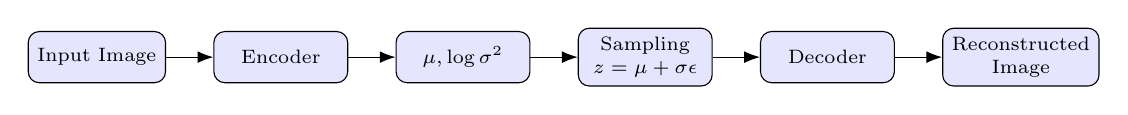
\begin{tikzpicture}[node distance=6mm]
\node[layer](a){Input Image};
\node[layer,right=of a](b){Encoder};
\node[layer,right=of b](c){$\mu,\log\sigma^2$};
\node[layer,right=of c](d){Sampling\\$z=\mu+\sigma\epsilon$};
\node[layer,right=of d](e){Decoder};
\node[layer,right=of e](f){Reconstructed\\Image};

\foreach \x/\y in {a/b,b/c,c/d,d/e,e/f}
\draw[arrow](\x)--(\y);
\end{tikzpicture}
\end{center}

%%%%%%%%%%%%%%%%%%%%%%%%%%%%%%%%%%%%%%%%%%%%%%%%%%%%%%%%%%%%
\section*{16. VAE Loss Function}

The VAE objective consists of two components.

\subsection*{Reconstruction Loss}

\[
\mathcal{L}_{rec}
=
-\mathbb{E}_{q_{\phi}(z|x)}
[\log p_{\theta}(x|z)].
\]

For normalized MNIST images, binary cross-entropy can be used.

\subsection*{KL Divergence}

\[
D_{KL}
\left(
q_{\phi}(z|x)\parallel p(z)
\right)
=
-\frac{1}{2}
\sum_j
\left(
1+\log\sigma_j^2-\mu_j^2-\sigma_j^2
\right).
\]

The total loss is

\[
\boxed{
\mathcal{L}_{VAE}
=
\mathcal{L}_{rec}
+
\mathcal{L}_{KL}
}
\]

where the prior is usually

\[
p(z)=\mathcal{N}(0,I).
\]

%%%%%%%%%%%%%%%%%%%%%%%%%%%%%%%%%%%%%%%%%%%%%%%%%%%%%%%%%%%%
\section*{17. VAE Implementation}

Use a small latent space so that it can be visualized.

Suggested latent dimension:

\[
z\in\mathbb{R}^{2}.
\]

The encoder should produce:

\[
\mu\in\mathbb{R}^{2},
\qquad
\log\sigma^2\in\mathbb{R}^{2}.
\]

The decoder maps

\[
z\rightarrow28\times28\times1.
\]

A compact architecture is:

\begin{center}
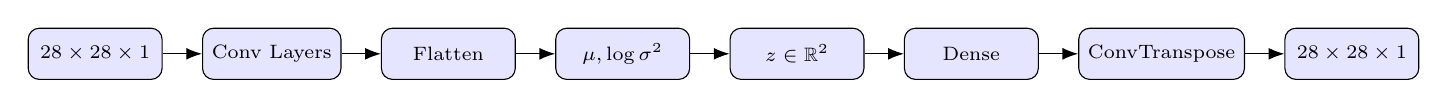
\begin{tikzpicture}[node distance=5mm]
\node[layer](a){$28\times28\times1$};
\node[layer,right=of a](b){Conv Layers};
\node[layer,right=of b](c){Flatten};
\node[layer,right=of c](d){$\mu,\log\sigma^2$};
\node[layer,right=of d](e){$z\in\mathbb{R}^2$};
\node[layer,right=of e](f){Dense};
\node[layer,right=of f](g){ConvTranspose};
\node[layer,right=of g](h){$28\times28\times1$};

\foreach \x/\y in {a/b,b/c,c/d,d/e,e/f,f/g,g/h}
\draw[arrow](\x)--(\y);
\end{tikzpicture}
\end{center}

%%%%%%%%%%%%%%%%%%%%%%%%%%%%%%%%%%%%%%%%%%%%%%%%%%%%%%%%%%%%
\section*{18. Exploring the VAE Latent Space}

Since the latent dimension is two, students can visualize the encoded test
images in a two-dimensional plane.

\textbf{Plot 6: VAE Latent Space}

\begin{itemize}
\item X-axis: $z_1$
\item Y-axis: $z_2$
\item Color/marker category: digit label
\end{itemize}

The labels are used only for visualization; they are not supplied to the VAE
during training.

\begin{figure}[H]
    \includegraphics[width=0.9\textwidth]{12.png}
    \caption{Plot 6: VAE latent space visualization of MNIST test images.}
\end{figure}

\textbf{Inference:} In the plot above, the latent space is represented in two dimensions for the test images of the MNIST database using various colors to denote the labels of the digits. It is noted that samples having the same digits form partially concentrated clusters, for example, for certain digits like 0, 1, and 9. Nevertheless, there is a significant overlap in various digit classes, especially in the center of the latent space. This phenomenon is brought about by the fact that the latent representation learned by the VAE is probabilistic and not separated into various classes.

%%%%%%%%%%%%%%%%%%%%%%%%%%%%%%%%%%%%%%%%%%%%%%%%%%%%%%%%%%%%
\section*{19. Generating New Images with the VAE}

Sample points from

\[
z\sim\mathcal{N}(0,I).
\]

Pass the sampled latent vectors through the decoder.

\textbf{Plot 7: Randomly Generated Images}

Generate at least 25 images using randomly sampled latent vectors.

Display them in a grid.

Students should determine:

\begin{itemize}
\item whether the generated images resemble handwritten digits;
\item whether digit shapes are recognizable;
\item whether there is visible variation among generated samples; and
\item whether some samples are ambiguous or unrealistic.
\end{itemize}
\begin{figure}[H]
    \includegraphics[width=0.75\textwidth]{13.png}
    \caption{Plot 7: Randomly generated images sampled from the VAE latent distribution.}
\end{figure}

\textbf{Inference:} 
The plot displays 25 samples produced by sampling latent vectors from the standard normal distribution and running them through the VAE decoder. The majority of the produced samples look like handwritten digits, and some of the digit shapes can be easily recognized. Variation in the produced samples is observed, which means that the VAE is able to generate different outputs and does not simply reproduce one output pattern. At the same time, some of the produced samples are blurry or ambiguous, and some of the digits are hard to recognize precisely. It happens due to the probabilistic nature of image generation by the VAE.
%%%%%%%%%%%%%%%%%%%%%%%%%%%%%%%%%%%%%%%%%%%%%%%%%%%%%%%%%%%%
\section*{20. Latent Space Interpolation}

Select two latent vectors:

\[
z_A,\qquad z_B.
\]

Construct

\[
z(\alpha)=(1-\alpha)z_A+\alpha z_B,
\qquad
\alpha\in[0,1].
\]

Use values such as:

\[
\alpha=
0,\;0.1,\;0.2,\ldots,1.
\]

Decode every interpolated vector.

\textbf{Plot 8: Latent Space Interpolation}

Display the decoded images in sequence.
\begin{figure}[H]
    \centering
    \includegraphics[width=\textwidth]{14.png}
    \caption{Plot 8: Latent space interpolation between two latent vectors.}
\end{figure}

\textbf{Inference:} The plot depicts the decoded images that are generated through interpolation between two latent vectors as $\alpha$ varies from 0 to 1. The digit varies smoothly throughout the process, with the transition between the images being smooth in terms of shape rather than occurring abruptly. This implies that points close together in the latent space learned by the network represent visually similar images. This is due to the VAE training a latent space that varies smoothly, and the decoder mapping latent points between the two points to produce corresponding images.

%%%%%%%%%%%%%%%%%%%%%%%%%%%%%%%%%%%%%%%%%%%%%%%%%%%%%%%%%%%%
\section*{21. Reconstruction Comparison Across Models}

Compare the three reconstruction-based models:
\begin{center}
\begin{tabular}{|l|c|c|c|c|}
\hline
\textbf{Model} & \textbf{MSE} & \textbf{MAE} & \textbf{SSIM} & \textbf{Parameters}\\
\hline
Fully Connected AE & 0.022764 & 0.060162 & 0.724705 & 211040\\
Convolutional AE & 0.002618 & 0.015085 & 0.973805 & 74497\\
Denoising CAE & 0.004622 & 0.021272 & 0.944603 & 74497\\
\hline
\end{tabular}
\end{center}

\begin{center}
\begin{tabular}{|l|c|}
\hline
\textbf{VAE Metric} & \textbf{Value}\\
\hline
Reconstruction Loss & 149.801590\\
KL Loss & 5.588442\\
Total Loss & 155.390030\\
Test MSE & 0.044398\\
Test MAE & 0.105164\\
Mean SSIM & 0.485619\\
\hline
\end{tabular}
\end{center}

%%%%%%%%%%%%%%%%%%%%%%%%%%%%%%%%%%%%%%%%%%%%%%%%%%%%%%%%%%%%
\section*{22. Required Plots}

The final report must contain the following plots:

\begin{enumerate}
\item Original image versus reconstructed image.
\item Training and validation loss for the basic autoencoder.
\item Fully connected AE versus convolutional AE reconstruction.
\item Clean versus noisy versus denoised images.
\item Noise level versus MSE/MAE/SSIM.
\item VAE latent-space visualization.
\item Randomly generated VAE images.
\item Latent-space interpolation.
\item Training/validation reconstruction loss for the VAE.
\item Reconstruction-error distribution on the test set.
\end{enumerate}

For plots containing multiple quantitative measures, use separate figures or
clearly labeled axes rather than placing incompatible scales on one axis.

%%%%%%%%%%%%%%%%%%%%%%%%%%%%%%%%%%%%%%%%%%%%%%%%%%%%%%%%%%%%
\section*{23. Reconstruction Error Distribution}

Calculate the per-image reconstruction error:

\[
e_i=
\frac{1}{D}
\sum_{j=1}^{D}
(x_{ij}-\hat{x}_{ij})^2.
\]

\textbf{Plot 9: Distribution of Reconstruction Errors}
\begin{figure}[H]
    \centering
    \includegraphics[width=0.9\textwidth]{15.png}
    \caption{Plot 9: Distribution of per-image reconstruction errors.}
\end{figure}

\textbf{Inference:} In this figure, the histogram displays the distribution of per-image reconstruction errors within the test set. Most of the reconstruction errors cluster somewhere between 0.03 and 0.07, with a majority at approximately 0.04 to 0.06. The distribution is somewhat dispersed, with a right-skewed tail reaching about 0.12. This implies that there are fewer images that have higher reconstruction errors than the rest. This could be attributed to the fact that those particular images contain digits of odd appearance or complex stroke patterns that are difficult to reconstruct through the use of the autoencoder.

%%%%%%%%%%%%%%%%%%%%%%%%%%%%%%%%%%%%%%%%%%%%%%%%%%%%%%%%%%%%
\section*{24. Required High-Error Image Analysis}

Select the five test images having the largest reconstruction errors.
\begin{center}
\begin{tabular}{|c|c|c|}
\hline
\textbf{Sample} & \textbf{Original} & \textbf{Reconstruction}\\
\hline
1 & Digit 5, Error = 0.117970 & Digit 5 reconstruction\\
2 & Digit 5, Error = 0.114688 & Digit 5 reconstruction\\
3 & Digit 2, Error = 0.109714 & Digit 2 reconstruction\\
4 & Digit 8, Error = 0.106810 & Digit 8 reconstruction\\
5 & Digit 5, Error = 0.106108 & Digit 5 reconstruction\\
\hline
\end{tabular}
\end{center}

\begin{figure}[H]
    \includegraphics[width=0.5\textwidth]{16.png}
    \caption{Five test images with the highest reconstruction errors and their corresponding reconstructions.}
\end{figure}

\textbf{Inference:}The five samples with the largest error rates are predominantly digits that have irregular handwriting style. The initial pictures show some irregularities with regard to the thickness, shapes, orientations, and structures of the strokes that do not match the most common styles of digit images used for training the VAE model. As a result, the reconstructions look smoother and, in some cases, represent an image closer to the general style of the digit than to the actual handwriting style used in the initial picture. It is possible to assume that the VAE manages to identify common digit structures but has difficulties with irregular ones.

%%%%%%%%%%%%%%%%%%%%%%%%%%%%%%%%%%%%%%%%%%%%%%%%%%%%%%%%%%%%
\section*{25. Consolidated Results}
\begin{center}
\begin{tabular}{|l|c|c|c|c|c|}
\hline
\textbf{Model} & \textbf{MSE} & \textbf{MAE} & \textbf{SSIM} & \textbf{Parameters} & \textbf{Time (s)}\\
\hline
FC Autoencoder & 0.022764 & 0.060162 & 0.724705 & 211040 & 25.889394\\
Conv. Autoencoder & 0.002618 & 0.015085 & 0.973805 & 74497 & 751.534856\\
Denoising CAE & 0.004622 & 0.021272 & 0.944603 & 74497 & 694.482783\\
VAE & 0.044398 & 0.105164 & 0.485619 & 485957 & 650.391763\\
\hline
\end{tabular}
\end{center}

The values must be obtained from the student's own execution.

%%%%%%%%%%%%%%%%%%%%%%%%%%%%%%%%%%%%%%%%%%%%%%%%%%%%%%%%%%%%
\section*{26. Required Inferences}

For every major plot, students must write a short inference containing:

\begin{enumerate}
\item What does the plot show?
\item What trend is observed?
\item Why might the observed trend occur?
\item What conclusion can be drawn?
\end{enumerate}


\subsection*{Effect of Latent Dimension on Reconstruction}
However, as the value of the latent dimension rises from 2 to 32, there is a fall in the value of the reconstruction MSE from 0.059498 to 0.023802, while SSIM rises from 0.272002 to 0.710337, indicating better reconstruction. However, there is an increase in the parameters from 210130 to 212080. However, the improvement is smaller for larger values of the latent dimension, and there is just a moderate improvement from the value of the latent dimension of 16 to 32.

\subsection*{Difference Between Fully Connected and Convolutional Reconstruction}
The convolutional autoencoder shows better reconstruction results compared to the fully connected autoencoder. In terms of MSE, it goes down from 0.022764 in case of the fully connected autoencoder to 0.002618 in case of the convolutional autoencoder, whereas SSIM goes up from 0.724705 to 0.973805. Convolutional structure retains better spatial information due to the use of convolutional filters. Thus, the convolutional autoencoder demonstrates better results with a smaller number of parameters in the current experiment.

\subsection*{Effect of Gaussian Noise Level}
With the increase of Gaussian noise from $\sigma = 0.1$ to $\sigma = 0.3$, the quality of reconstruction falls. The MSE goes up from 0.003628 to 0.007102, and the MAE goes up from 0.017821 to 0.029666. In addition, the SSIM goes down from 0.959859 to 0.863580. Noise causes bigger distortion of the input image; therefore, it is harder to reconstruct the original image by the denoising autoencoder.

\subsection*{Ability of the Denoising Autoencoder to Recover Image Structure}
The Denoising Autoencoder is capable of extracting the major structural components of the input digits and ignoring a significant amount of the introduced noise. The denoised output images retain their ability to be identified and contain the major structure of the original clean images. This is due to the fact that the Denoising Autoencoder model trains by taking the noisy images as input and the clean images as target outputs.

\subsection*{Characteristics of the VAE Latent Distribution}
The latent space obtained by the VAE is continuous in nature and based on probability instead of having a fixed deterministic vector for each data point. The parameters of the distribution are provided by the encoder, and sampling takes place using the parameters of this distribution. The term KL-divergence works toward keeping the learned distribution similar to the normal prior.

\subsection*{Structure of the Two-Dimensional VAE Latent Space}
VAE latent space is 2D in nature and exhibits partially disjoint zones for different classes of digits, even though some amount of overlapping takes place. This means that the latent space has captured the features of the digits in such a way that there is no forced separation between the digits’ classes. The overlapping happens due to the fact that the VAE is trained more for reconstruction and not for classification.

\subsection*{Quality and Diversity of Generated Samples}
In general, the output from the trained VAE looks like handwritten digits with variations in terms of shapes and orientations. Some of the output images may be somewhat ambiguous for latent vectors, which do not necessarily correspond to well-represented images in the training set. Variations among different generated images indicate that VAE is capable of generating a variety of outputs rather than just reproducing training images.

\subsection*{Smoothness of Latent-Space Interpolation}
From the interpolation of the latent space, we observe that the images produced vary gradually while moving from one point to another in the latent space. This is seen in terms of the structures of digits changing gradually and not suddenly. This shows that points near each other in the latent space can represent similar features in the image. This smooth transition is also attributed to the fact that the latent space is continuously probabilistic in nature.

\subsection*{Relationship Between Reconstruction Error and Visual Quality}
It is evident from the distribution plot of the reconstruction error that a majority of the samples have a low value of reconstruction error, whereas some samples have high values of reconstruction error. The top five values of the reconstruction error for these samples are 0.117970, 0.114688, 0.109714, 0.106810, and 0.106108. In some cases, high reconstruction errors can be due to unusual handwriting, thickness of the stroke, orientation, or shape of the images. Hence, a lower reconstruction error implies the presence of good visual structure.

\subsection*{Differences Between Deterministic and Probabilistic Latent Representations}
While standard autoencoders make use of deterministic latent representations wherein each input is transformed into a fixed latent vector, the VAE creates a probability distribution where from the latent vectors can be generated. While the deterministic representations aim at conserving the information for reconstruction, the probabilistic representations allow the creation of a continuous latent space that makes sampling, interpolation, and generation possible. The performance measures for the two models in terms of their respective results are MSE = 0.002618, SSIM = 0.973805 for the convolutional autoencoder, and MSE = 0.044398, SSIM = 0.485619 for the VAE.
%%%%%%%%%%%%%%%%%%%%%%%%%%%%%%%%%%%%%%%%%%%%%%%%%%%%%%%%%%%%
\section*{27. Additional Latent-Dimension Study}

Repeat the basic autoencoder using:

\[
d_z\in\{2,8,16,32\}.
\]

Report:

\begin{center}
\begin{tabular}{|c|c|c|c|}
\hline
Latent Dimension & MSE & SSIM & Parameters\\
\hline
2  & 0.059498 & 0.272002 & 210130\\
8  & 0.038209 & 0.560091 & 210520\\
16 & 0.026819 & 0.678831 & 211040\\
32 & 0.023802 & 0.710337 & 212080\\
\hline
\end{tabular}
\end{center}
\textbf{Plot 10: Latent Dimension vs. Reconstruction MSE}

\begin{figure}[H]
    \centering
    \includegraphics[width=0.6\textwidth]{17.png}
    \caption{Latent Dimension vs. Reconstruction MSE}
\end{figure}

\textbf{Inference:}
As the latent dimension rises from 2 to 32, the reconstruction MSE falls from 0.059498 to 0.023802 and the SSIM value rises from 0.272002 to 0.710337, indicating an increase in the quality of reconstruction. However, the parameters have also increased from 210130 to 212080. The increase becomes small as we go further up to larger values of latent dimensions, with only modest improvement in values from latent dimension 16 to 32.

%%%%%%%%%%%%%%%%%%%%%%%%%%%%%%%%%%%%%%%%%%%%%%%%%%%%%%%%%%%%
\section*{28. Discussion Questions}

\begin{enumerate}

\item \textbf{What is an autoencoder?}
The autoencoder is an artificial neural network whose task is to reproduce its inputs on its outputs. The input data is compressed by the encoder and then decoded back into the original form by the decoder.
\item \textbf{What is the purpose of the encoder?}
The encoder converts input images into a lower-dimensional latent representation that captures the key features of that input. 

\item \textbf{What is the purpose of the decoder?}
The original image is reconstructed by the decoder based on the encoder’s latent representation.

\item \textbf{What is a latent representation?}
Latent representation can be defined as the compressed form of the input obtained through the encoder. It contains the significant information that is necessary for the decoder to reconstruct the input.
\item \textbf{Why is the latent representation usually smaller than the input?}
However, the latent representation is normally of lower dimension than the data input as this will enable the model to extract the most important characteristics of the input rather than copy the input entirely.

\item \textbf{What happens when the latent dimension is too small?}
If the dimensionality of the hidden variable is not enough, then there will not be enough capacity in the model for encoding all necessary information from the input data.
\item \textbf{What happens when the latent dimension is increased?}
As the latent space dimension is increased, the network has greater capability to retain information and therefore has better performance in reconstruction. In the case study, MSE was reduced from 0.059498 at dimension 2 to 0.023802 at dimension 32, while SSIM was improved from 0.272002 to 0.710337. Nevertheless, the number of parameters is also increased.

\item \textbf{Why can a convolutional autoencoder preserve spatial?
The convolutional autoencoder works directly with the two-dimensional structure of the image using convolutional filters, which preserve local spatial relationships among neighboring pixels and learn local image features effectively.nformation more effectively?}


\item \textbf{Differentiate an autoencoder and a denoising autoencoder.}
An autoencoder is trained in such a way that it reconstructs the input from the input. In the case of a denoising autoencoder, however, the input provided is a corrupted image while the target used for training is the clean image.

\item \textbf{Why is the clean image used as the target in denoising?}
The clean image is employed as the target since this helps the model learn how to reconstruct the actual image, instead of copying the noise inherent in the noisy image.

\item \textbf{What happens when the noise level is increased?}
As the amount of noise is increased, reconstruction becomes more challenging. In this case, Gaussian noise with $\sigma=0.1$, $0.2$ and $0.3$ gave increasing MSE of 0.003628, 0.004630 and 0.007102 while the value of SSIM was reduced from 0.959859 to 0.863580.

\item \textbf{Why are MSE, MAE and SSIM useful for image reconstruction?}
MSE is the measure of the average square of the differences between the original and reconstructed images, while MAE is the measure of the average of the absolute values of the differences. SSIM evaluates the similarity in the structure of the image.

\item \textbf{What is a Variational Autoencoder?}
A variational autoencoder (VAE) is a generative deep neural network where a latent probability distribution of the input data is learned. A VAE comprises an encoder, a sampling step, and a decoder.
\item \textbf{How does a VAE differ from a conventional autoencoder?}
While a standard autoencoder learns the latent representation directly from the input, a Variational Autoencoder (VAE) infers the distribution of the parameters in the latent space and generates samples from that distribution. A KL-divergence term is included in the VAE architecture for regularization of the latent distribution.
\item \textbf{Why does a VAE learn a distribution instead of a single latent vector?}
The learning of a distribution results in a continuous latent space that can be sampled to generate new latent samples. The VAE is therefore able to not only reconstruct but also to generate and interpolate.
\item \textbf{What is the reparameterization trick?}
Reparameterization trick helps the VAE draw samples from the latent distribution and remain differentiable during the training process. This means that instead of drawing samples z from the distribution that has been learnt, the latent vector is written in terms of the learned mean and standard deviation.

\item \textbf{Why is $\epsilon$ sampled from a standard normal distribution?}
The value of $\epsilon$ is drawn from the standard normal distribution to introduce the random variations in the latent space in a controllable and differentiable way. This is then used along with the learned mean and variance to get the latent variable.

\item \textbf{What is the role of KL divergence in the VAE loss?}
KL divergence acts as a regularization technique to ensure that the latent distribution remains close to the selected prior distribution. This makes it possible to generate a continuous latent space for sampling purposes.

\item \textbf{What is the prior distribution used in the VAE?}
The prior distribution for the VAE is the standard Gaussian distribution, denoted by

\[
p(z)=\mathcal{N}(0,I).
\]

The KL divergence component forces the learned distribution to stay close to the prior distribution.

\item \textbf{Why is a two-dimensional latent space useful for visualization?}
The use of a two-dimensional latent space facilitates visualization of the representation space in a two-dimensional graph, which helps to see the clustering, overlap, and the overall pattern of the representations of different digits.
\item \textbf{What does latent-space interpolation demonstrate?}
Interpolation in the latent space verifies whether the learned latent space is continuous. The result of the experiment showed that the generated images were continuously varying from one selected point to the other in the latent space.

\item \textbf{Why can a VAE generate new images?}
In a VAE, the latent space is learned as a probabilistic latent space whose values tend to conform to some prior distribution. Therefore, one can sample new latent vectors from the learned distribution and decode them into images.

\item \textbf{Why might some VAE-generated images be unclear?}

The decoded images can sometimes appear vague because the decoder will be getting samples from areas where there is no representation of strong training samples. The probabilistic characteristic of the VAE and the balance between reconstruction and generation can cause blurriness in the output images.
\item \textbf{What is the difference between reconstruction and generation?}
reconstruction includes encoding of the input image and then decoding it to recreate the image. The process of generation on the other hand includes sampling of a latent image and then decoding the sample to generate a new image.

\item \textbf{Why should test images remain unseen during training?}
The test images must not be seen by the model when it is trained because the test set acts as an unbiased measure of the ability of the model to generalize on unseen images. Seeing the test images while training causes data leakage.

\end{enumerate}
%%%%%%%%%%%%%%%%%%%%%%%%%%%%%%%%%%%%%%%%%%%%%%%%%%%%%%%%%%%%
\section*{29. Additional Exercises -- Discussion Points}

\begin{enumerate}

\item \textbf{Train the convolutional autoencoder with latent dimensions of 4, 8, 16 and 32 and compare reconstruction quality.}
The goal here would be to look at the relationship between the ability of the convolutional autoencoder and the reconstruction of images. Reconstruction efficiency could be determined through MSE, MAE, and SSIM. Having a low latent dimension will mean high compression efficiency but could also mean that significant spatial and structural data will be omitted. Higher latent dimensions will result in better efficiency in preserving features and therefore higher efficiency in reconstruction. There will be a point where having higher latent dimension will no longer yield significant gains.

\item \textbf{Compare Gaussian noise and salt-and-pepper noise using the same denoising architecture.}

In this task, we will explore if the denoising autoencoder behaves differently when subjected to various noise types. While Gaussian noise represents random values within a range, salt-and-pepper noise represents individual pixels with very high and low intensity. This way, by keeping the architecture of the model and the level of noise similar, we can compare the results based on MSE, MAE, and SSIM. The dissimilar performance would show that the efficiency of denoising is influenced not only by the level but also the properties of the noise.

\item \textbf{Train the denoising autoencoder using two different noise levels and compare SSIM.}
In this experiment, the effect of an increase in corruption on the quality of reconstruction images structurally will be assessed. The SSIM metric is very relevant since it measures structural similarity instead of the difference between pixels. If there is a reduction in the SSIM metric at a high noise level, it shows that the increase in corruption leads to difficulties in reconstructing the structural image. This way, it will be possible to identify the noise level when the denoising model starts losing structural information.
\item \textbf{Replace the convolutional decoder with transposed convolutions and compare the reconstructions.}
This exercise will look at how the architecture of the decoder influences image reconstruction. The decoder that uses transposed convolutions will be able to learn the spatial upsampling, while the original architecture may perform upsampling and convolution separately. Both methods need to be compared based on their performance using the reconstruction metrics, but also in terms of visual quality. Apart from the MSE, MAE, and SSIM, visual comparison is necessary to spot any differences.

\item \textbf{Implement a VAE with latent dimension 2 and 8 and compare the latent representations.}
The purpose of this experiment is to understand the effects of latent space dimension on the information obtained through the VAE. A latent space of two dimensions is easily visualized and can give insights into the clusters, overlapping, and continuity between various digit classes. By increasing the dimension to 8, there will be increased latent space which will help to capture more information from the input images. This experiment will show the relationship between visualization and latent representation capacity.

\item \textbf{Investigate the effect of increasing the KL-loss contribution.}
KL-divergence helps in regulating how much the trained latent distribution should stay close to the prior distribution. The greater its weight, the greater the effect of the latent space regularization. This will make the latent space smoother and structured, although too much regularization will limit the amount of information that can be used for reconstruction. It is therefore necessary to evaluate the impact of the parameter using both the reconstruction metrics and the latent space structure.
\item \textbf{Generate a larger grid of VAE samples and discuss diversity.}More sample generation will provide a more complete picture of the variation that the VAE has learned. The samples generated should be inspected for variation in digit, stroke width, orientation, shape, and other visual variation. A good generative model will have a variety of samples that are sufficiently varied from each other while retaining the properties of the MNIST data. Repetitive or duplicate samples could point to lack of variation, and very distorted samples could suggest that there is underrepresentation in parts of the latent space.

\item \textbf{Select two digit regions in the latent space and perform interpolation.}
The purpose of this exercise is to check whether continuous changes are possible through the learned latent space. It is possible to choose two latent points for different digits and generate the intermediate latent vectors. Decoded images have to be analyzed to see whether the digit form changes in a smooth or a drastic way. Smooth transitions will mean that there are continuous meaningful points in the latent space, whereas drastic changes and very distorted images will suggest otherwise.

\end{enumerate}
%%%%%%%%%%%%%%%%%%%%%%%%%%%%%%%%%%%%%%%%%%%%%%%%%%%%%%%%%%%%
\section*{30. Expected Outcome}

At the end of the experiment, students should be able to demonstrate the
complete image-representation and reconstruction pipeline:

\[
\boxed{
\text{Image}
\rightarrow
\text{Encoder}
\rightarrow
\text{Latent Representation}
\rightarrow
\text{Decoder}
\rightarrow
\text{Reconstructed Image}
}
\]

They should also demonstrate denoising:

\[
\boxed{
\text{Clean Image}
\rightarrow
\text{Noise}
\rightarrow
\text{Denoising Autoencoder}
\rightarrow
\text{Recovered Image}
}
\]

and variational generation:

\[
\boxed{
\text{Image}
\rightarrow
(\mu,\sigma)
\rightarrow
z
\rightarrow
\text{Decoder}
\rightarrow
\text{Generated/Reconstructed Image}
}
\]

The final report should contain both quantitative evaluation and visual
analysis. Numerical performance values must be obtained from the student's
own execution.

%%%%%%%%%%%%%%%%%%%%%%%%%%%%%%%%%%%%%%%%%%%%%%%%%%%%%%%%%%%%
\section*{31. References}

\begin{enumerate}
\item Ian Goodfellow, Yoshua Bengio and Aaron Courville,
\emph{Deep Learning}, MIT Press, 2016.

\item Diederik P. Kingma and Max Welling,
``Auto-Encoding Variational Bayes,'' ICLR, 2014.

\item Pascal Vincent et al.,
``Stacked Denoising Autoencoders: Learning Useful Representations in a Deep
Network with a Local Denoising Criterion,'' Journal of Machine Learning
Research, 2010.

\item Yann LeCun, Corinna Cortes and Christopher J. C. Burges,
``MNIST Handwritten Digit Database.''

\item TensorFlow Documentation:
\url{https://www.tensorflow.org}

\item Keras Documentation:
\url{https://keras.io}

\item scikit-image Documentation:
\url{https://scikit-image.org}
\end{enumerate}

\end{document}
